%!TEX root = ../exa-ma-deliverables.tex
\chapter{Application Demonstrators and Co-design with Exa-DI}
\label{chap:exadi-demonstrators}
\label{sec:pc5:demonstrator-context}

\providecommand{\ExaDIRef}[3]{\hyperref[#1]{#2}}

An application demonstrator combines numerical methods, software and
datasets in a workflow that addresses a scientific, societal, environmental
or industrial question. The \ExaDIRef{chap:applications}{mini-applications and benchmarks}{https://exa-ma.numpex.fr/deliverables.html}
exercise the methods, kernels and stages these workflows depend on.

\href{https://numpex.org/exadi-development-and-integration/}{Exa-DI (PC5)}
coordinates co-design across NumPEx. Application teams bring their
requirements to thematic working groups with Exa-MA, Exa-SoFT, Exa-DoST
and Exa-AToW. The Computational Data Team (CDT) works with them to isolate
shared algorithmic motifs in proxy applications, benchmark methods, and
package and deploy reusable software. Application runs guide the next
iteration of development.

\Cref{tab:exadi-demonstrators} presents the three Exa-DI demonstrators
whose development involves Exa-MA (PC1) in this report. Their co-design
activities also involve other NumPEx projects.

\begin{table}[H]
\centering\small
\caption{Exa-DI (PC5) demonstrators and their links to Exa-MA (PC1).}
\label{tab:exadi-demonstrators}
\begin{tabularx}{\linewidth}{@{}>{\raggedright\arraybackslash}p{0.22\linewidth}
  >{\raggedright\arraybackslash}p{0.31\linewidth}
  >{\raggedright\arraybackslash}X@{}}
\toprule
\textbf{Demonstrator} & \textbf{Development and co-design} & \textbf{Exa-MA contributions}\\
\midrule
\hyperref[sec:pc5:ktirio-urban-building]{Ktirio Urban Building} &
University of Strasbourg (Cemosis). Co-funding from HiDALGO2 (50\%)
and Exa-DI (50\%). &
WP1 geometry, ray tracing and field transfer. WP6 ensemble execution and
uncertainty quantification. WP7 deployment and benchmarking.\\
\addlinespace
\hyperref[sec:pc5:funtides]{FUnTiDES} &
Inria Makutu and an energy-sector partner. Co-design with the CDT in
Exa-DI's high-order discretisation working group (WG1). &
WP1 high-order wave discretisation and portable operator studies.
WP7 application benchmarking and co-design coordination.\\
\addlinespace
\hyperref[sec:pc5:samurai]{Samurai} &
HPC@Maths, CMAP, École polytechnique. Co-design with Dyablo (CEA)
and the CDT in the Exa-DI mesh-adaptation working group (WG3). &
WP1 adaptive Cartesian meshes and high-order coupling verification.
WP7 benchmarking coordination.\\
\bottomrule
\end{tabularx}
\end{table}

\clearpage
\section{Ktirio Urban Building}
\label{sec:pc5:ktirio-urban-building}

\begin{FicheMetadataTable}[Ktirio Urban Building demonstrator profile.]
Domain & Urban energy, adaptation to extreme heat and building renovation. \\
Application team & Cemosis, University of Strasbourg. \\
Co-design and funding & Exa-DI (PC5) and HiDALGO2 co-fund the demonstrator equally.
HiDALGO2 is supported by the EuroHPC JU under grant 101093457. \\
Exa-MA contributions & WP1 geometry, distributed ray tracing and field
transfer. WP6 ensemble execution and uncertainty quantification.
WP7 software deployment, co-design and benchmarking. \\
Software and data & \href{https://kub.ktirio.fr/}{Ktirio Urban Building},
\ExaDIRef{sec:Feelpp:software}{Feel++}{https://feelpp.org/},
Ktirio-Geom, \ExaDIRef{sec:CGAL:software}{CGAL}{https://www.cgal.org/},
Modelica/FMI and preCICE. \href{https://ckan.hidalgo2.eu/dataset/ktirio-cases}{City datasets and model configurations}. \\
Reference cases & Tokyo terrain (\nolinkurl{BM-FEEL-KTIRIO-01}),
Paris 8\,km on Discoverer and Strasbourg heat exposure on Gaya. \\
\end{FicheMetadataTable}

\subsection{Context and objectives}

Which dwellings are most exposed during a heatwave? Which renovations
would reduce that exposure, and how would they change electricity demand?
Ktirio Urban Building addresses these questions at the scale of a
neighbourhood or city. Buildings under the same weather can respond
differently because of their construction, use, orientation and shading.
The demonstrator combines the geometry of an urban district with a thermal
model for each building to estimate those differences.

Proofs of concept with social housing providers use maps of indoor heat
exposure to prioritise buildings for field investigation and identify
where better building data are needed. The same workflow supports energy
planning studies with local authorities and the electricity sector, where
the objective is to compare the timing and magnitude of demand under
different weather or renovation scenarios. These cases connect building
time series to decisions about a housing portfolio or a district.
\ExaDIRef{sec:management-year-4}{D0.2 describes the collaborations.}{https://exa-ma.numpex.fr/deliverables.html}

The HiDALGO2 implementation work at Strasbourg is led by
Christophe Prud'homme with Vincent Chabannes, Javier Cladellas,
Philippe Pinçon and Gwennolé Chappron. The
\href{https://doi.org/10.1007/978-3-031-85703-4_2}{PPAM 2024 study}
describes the architecture and its deployment on EuroHPC systems
\cite{prudhomme_ktirio_2024}.

\subsection{Methods and HPC implementation}

\paragraph{Geometry and solar radiation (WP1).}
Ktirio-Geom uses CGAL to turn elevation and geographic data into
a mesh of buildings and terrain. The
\ExaDIRef{sec:app:specs:app-feelpp-ktirio-geom}{WP1 terrain and remeshing work}{https://kub.ktirio.fr/}
builds tiles in parallel and assembles a surface mesh with features
such as roads and water bodies. This mesh locates the buildings and
represents the surfaces that can obstruct sunlight. For each sun
direction, the
\ExaDIRef{sec:Feelpp:implementation-2026:bvh}{Feel++ distributed ray tracer}{https://github.com/feelpp/feelpp/releases/tag/v0.112.0}
uses a hierarchy of bounding boxes to find candidate MPI partitions,
then tests their local triangles for occlusion. The resulting solar
masks determine the direct solar gains used by the thermal models.

\paragraph{Weather and urban airflow (WP1 and WP7).}
The demonstrated WRF interface supplies spatially varying weather
to individual buildings in Strasbourg. The Lingolsheim study used
building surface temperatures to drive an airflow simulation. Resolving building--air
feedback requires exchanging surface temperatures and heat fluxes
with an urban airflow solver on its own mesh and time grid. The
\ExaDIRef{sec:Feelpp:implementation-2026:precice}{in-memory preCICE interface}{https://github.com/feelpp/feelpp/releases/tag/v0.112.0}
uses consistent temperature mapping and conservative flux transfer
in the heated-plate test with OpenFOAM. StationReplay exercises
the Ktirio side of the exchange with prescribed weather.
The next integration step with Széchenyi István University is to
close the two-way feedback loop at district scale with OpenFOAM or
RedSIM (HiDALGO2 D5.8 and D5.2).

A location dataset holds the urban geometry, the building stock and
the weather. The separately versioned simulator dataset contains
executable Modelica models packaged as Functional Mock-up Units
(FMUs). Ktirio assigns these to the buildings and runs them in
parallel through Feel++ using the Functional Mock-up Interface (FMI).
The Ktirio Dashboard shows the results as time series and maps
(\cref{fig:ktirio-ecosystem}).

\begin{figure}[!htb]
  \centering
  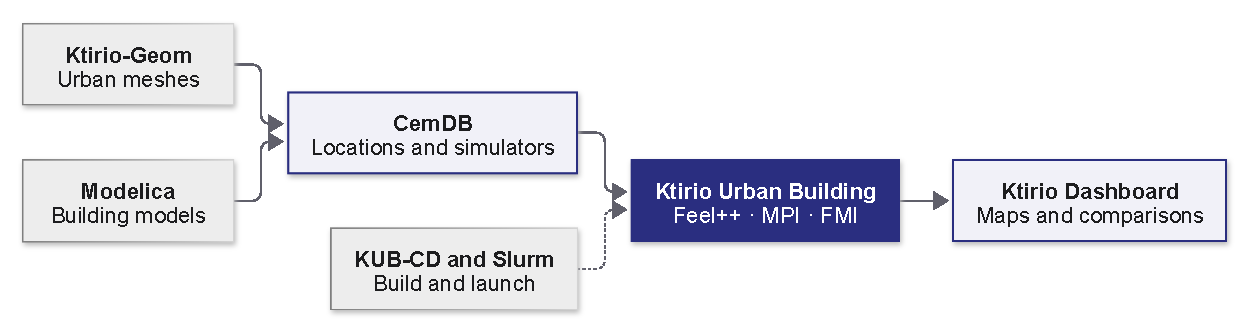
\includegraphics[width=\linewidth]{graphics/ktirio/ecosystem.pdf}
  \caption{Ktirio tools for preparing, running and analysing an urban building study.}
  \label{fig:ktirio-ecosystem}
\end{figure}

\paragraph{Ensembles and decision indicators (WP6).}
Material properties and building use are uncertain, particularly when a
study covers thousands of existing buildings. Ktirio runs the same city
for a sample of plausible inputs. A scenario set specifies the cases
to compare, a scenario lock records the resolved inputs and versions,
and an ensemble plan defines the parameter draws, computing resources
and outputs (\cref{fig:ktirio-scenario}). The run manifest records what
was executed. Several samples run concurrently
in separate MPI groups. The
\ExaDIRef{sec:wp6:ensemble-streaming}{WP6 statistical workflow}{https://kub.ktirio.fr/}
computes means, exceedance probabilities and quantiles from the ensemble.
For district-level quantities, it aggregates buildings within each
realisation before computing ensemble statistics, retaining the dependence
between buildings that share the same conditions.

\begin{figure}[H]
  \centering
  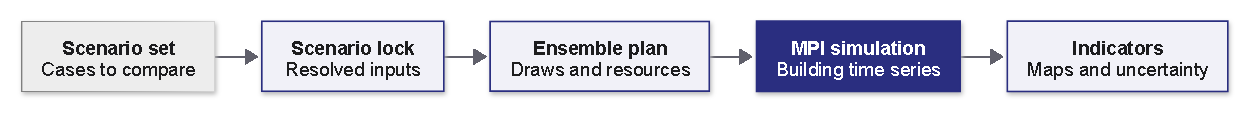
\includegraphics[width=\linewidth]{graphics/ktirio/scenario.pdf}
  \caption{From the scenarios and their resolved inputs to indicators computed across an ensemble.}
  \label{fig:ktirio-scenario}
\end{figure}

\paragraph{Data movement and output (WP1, WP6 and WP7).}
The Paris run uses a bounded number of concurrent HDF5 readers to
load an already partitioned city mesh. During a campaign such as
Strasbourg, dedicated statistical ranks accumulate summaries while
the building models run. Exact quantiles can require retaining
selected values. Mergeable sketches bound the amount of data stored for
approximate quantiles. These choices determine which indicators can be
computed in situ and which trajectories need to be written for later
analysis. The
\ExaDIRef{sec:app:specs:app-feelpp-io}{Feel++ I/O benchmark}{https://exa-ma.numpex.fr/deliverables.html}
measures preparation, writing and reloading separately.

The ReproHPC study links versioned software, input data and run records.
It uses a short Ktirio rerun to check the execution chain and inspects
archived files to verify the identity and integrity of the saved
outputs \cite{cladellas_layered_2026}.

\subsection{Results and benchmarks}
\label{sec:pc5:ktirio-results}

% HiDALGO2 D5.7, sec. 3.1 and fig. 3; D5.8, sec. 4 and sec. 8.1--8.5.
% HiDALGO2 D3.3, UNISTRA contribution, Paris 8 km campaign.
% HiDALGO2 D4.10 v0.4, sec. 4.2.4 and tables UB2--UB4.
\begin{table}[!htbp]
\centering\small
\caption{Ktirio Urban Building studies and their main results.}
\label{tab:exadi-ktirio-results}
\begin{tabularx}{\linewidth}{@{}>{\raggedright\arraybackslash}p{0.23\linewidth}
  >{\raggedright\arraybackslash}X@{}}
\toprule
\textbf{Study} & \textbf{Result}\\
\midrule
Tokyo terrain &
For an 81-tile domain of about 20\,km$^2$, tile generation fell from
117.18\,s with one worker to 4.57\,s with 32 workers on a Gaya node
(\ExaDIRef{sec:app:specs:app-feelpp-ktirio-geom}{\nolinkurl{BM-FEEL-KTIRIO-01}}{https://kub.ktirio.fr/}).\\
\addlinespace
Chicago reconstruction &
Buildings, roads, vegetation and water surfaces were reconstructed
at several scales and illustrated in a
\href{https://www.cemosis.fr/en/news/chicago-numpex-sc2026/}{NumPEx poster at SC26}.\\
\addlinespace
Paris 8\,km on Discoverer &
The Building-only run simulated 207,624 buildings on 32\,768 MPI
ranks. It used 68,207,038 mesh triangles and traced 471,821,112
solar rays in 14\,min 55\,s wall time, with field output disabled.\\
\addlinespace
Strasbourg heat exposure &
384 Monte Carlo realisations across 4,169 buildings produced
1,600,896 building evaluations. The production runs used
21,322.4 allocated core-hours on Gaya and produced 167.19\,GB
of outputs, including saved trajectories and run files
(HiDALGO2 D4.10).\\
\addlinespace
Building physics and energy &
Annual heating and cooling loads met ANSI/ASHRAE Standard~140
acceptance criteria for the BESTEST cases evaluated (HiDALGO2 D5.8).
A \href{https://www.hidalgo2.eu/wp-content/uploads/2025/06/HiDALGO2_D5.7-Implementation-Report-on-Pilot-Applications_v1.0.pdf}{separate Paris energy study}
mapped useful energy for more than 160,000 buildings (D5.7, Fig.~3).\\
\bottomrule
\end{tabularx}
\end{table}

\paragraph{Paris.}
\Cref{fig:ktirio-paris-mesh} shows the geometry used for the Paris
case, which covers an 8\,km radius around Notre-Dame. In the matched
mask tests, increasing the number of MPI ranks from 8\,192 to 16\,384
reduced the Building-only mask phase from 24.59\,s to 15.33\,s.
The Allfaces variant traced about 2.6 times as many rays per sunlit
step and its mask time stayed near 50\,s
(\ExaDIRef{tab:Feelpp:solar-mask-discoverer}{Discoverer phase timings}{https://exa-ma.numpex.fr/highlights/ktirio-paris-8km.html}).
The Building-only case reached 32\,768 ranks with the bounded mesh
reader.

\begin{figure}[!htb]
  \centering
  \begin{subfigure}[t]{0.485\linewidth}
    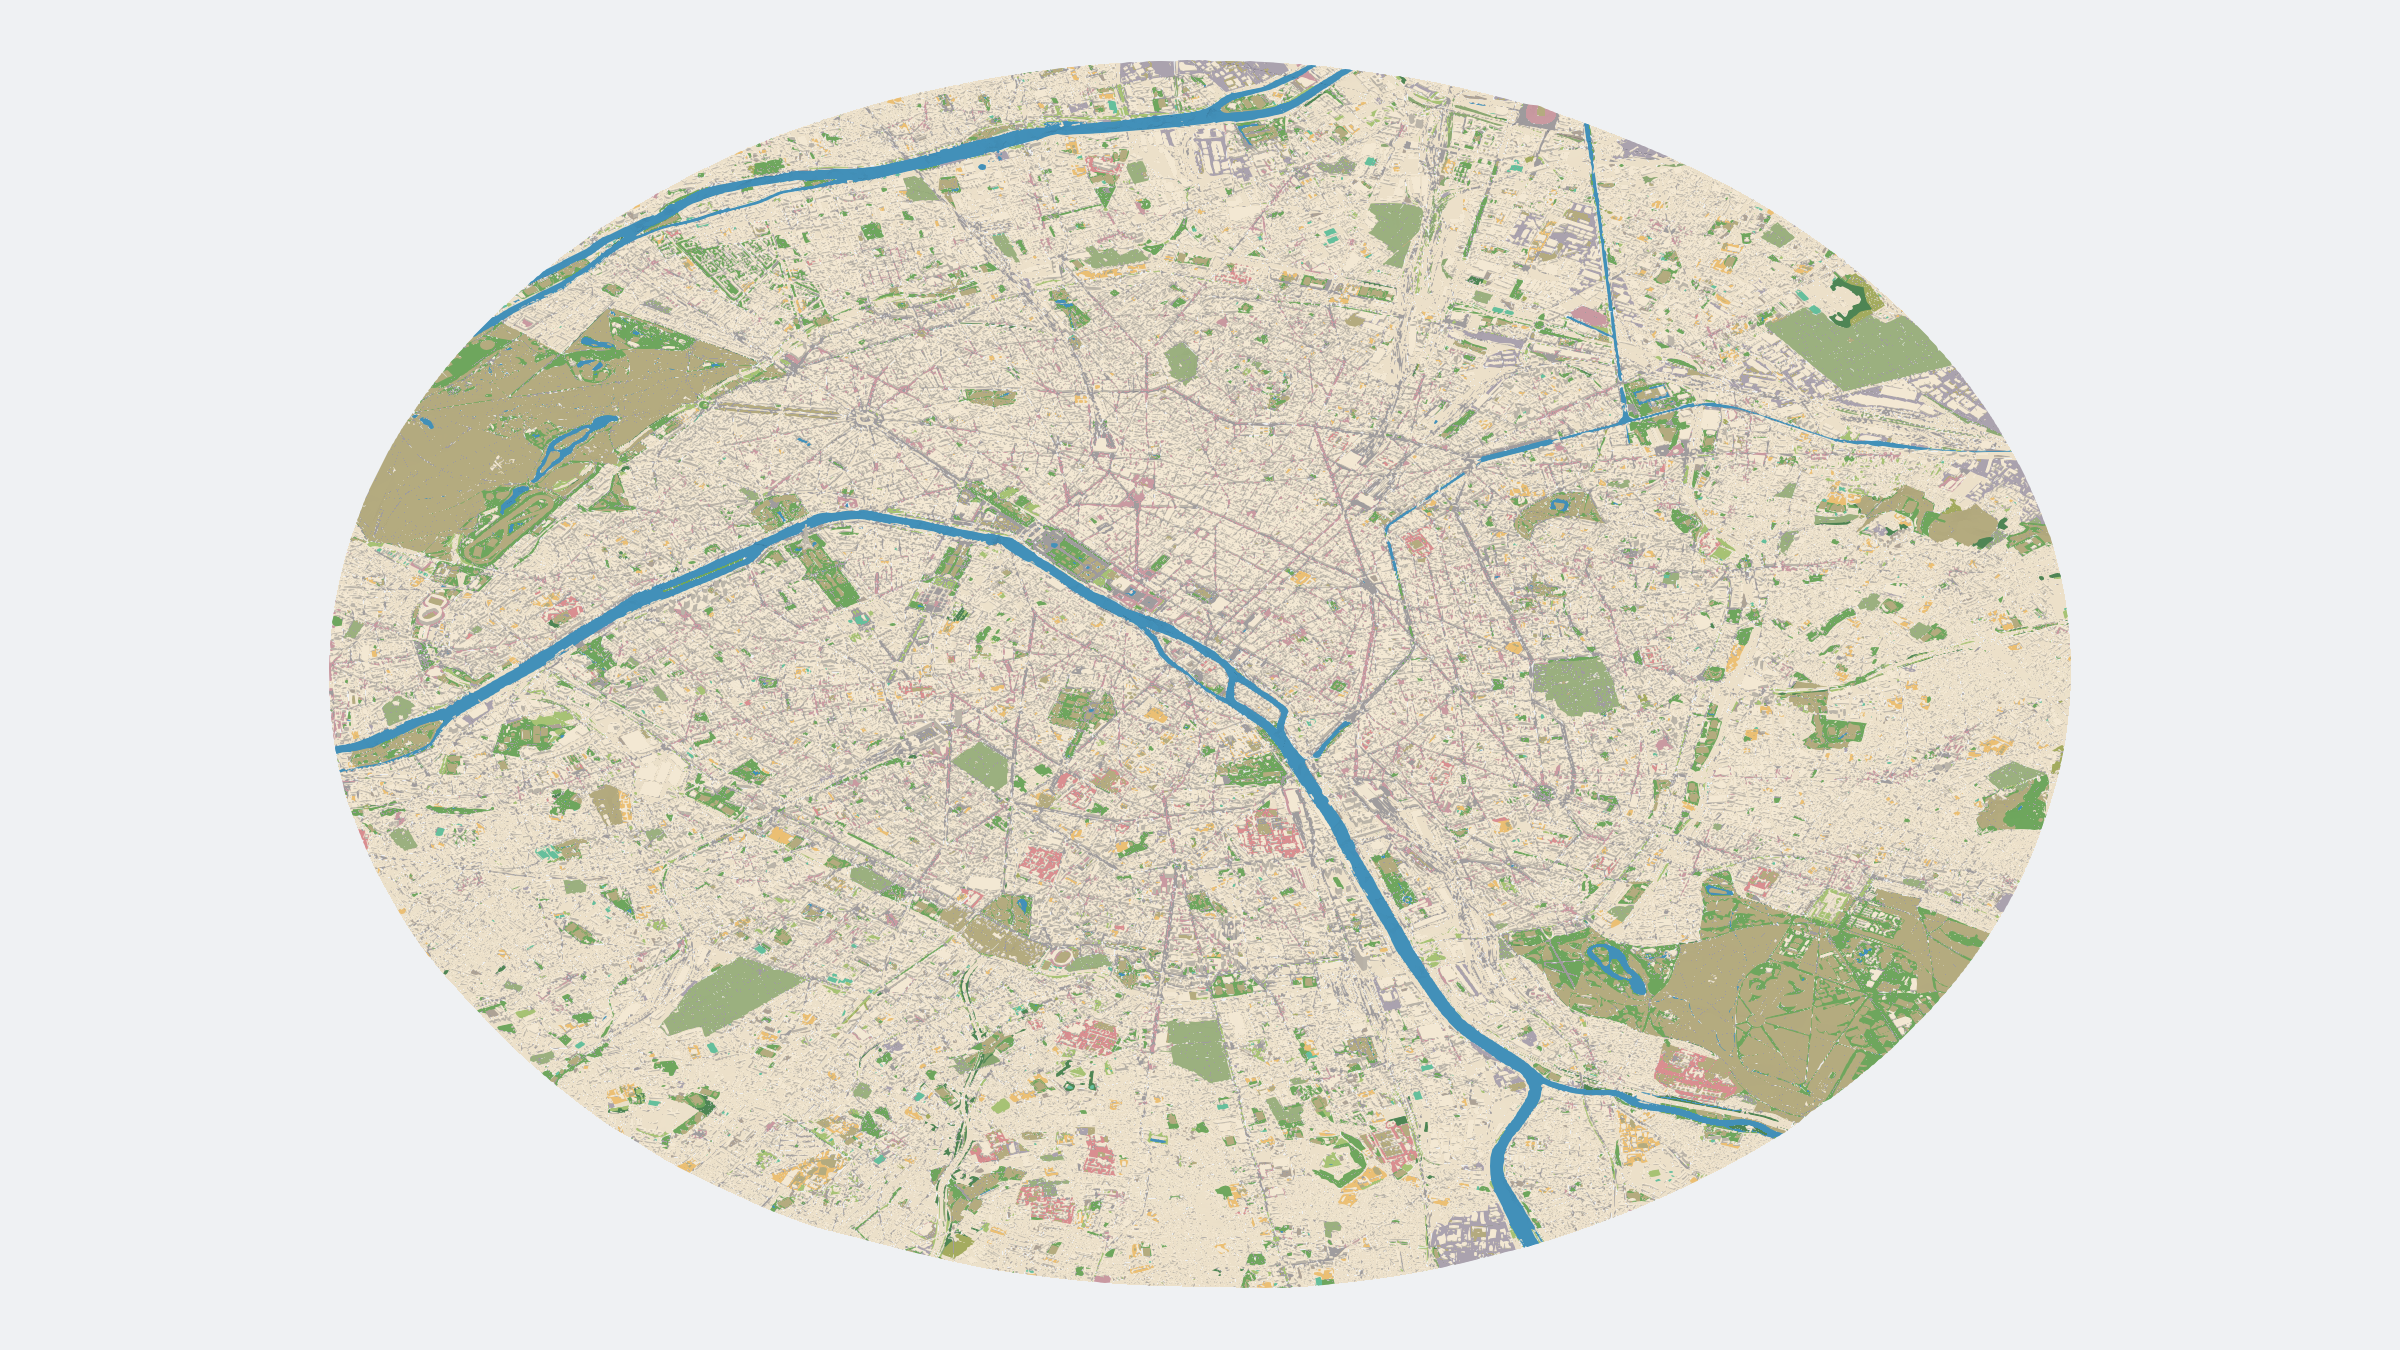
\includegraphics[width=\linewidth]{graphics/ktirio/paris-8km.png}
    \caption{The Paris 8\,km domain.}
  \end{subfigure}\hfill
  \begin{subfigure}[t]{0.485\linewidth}
    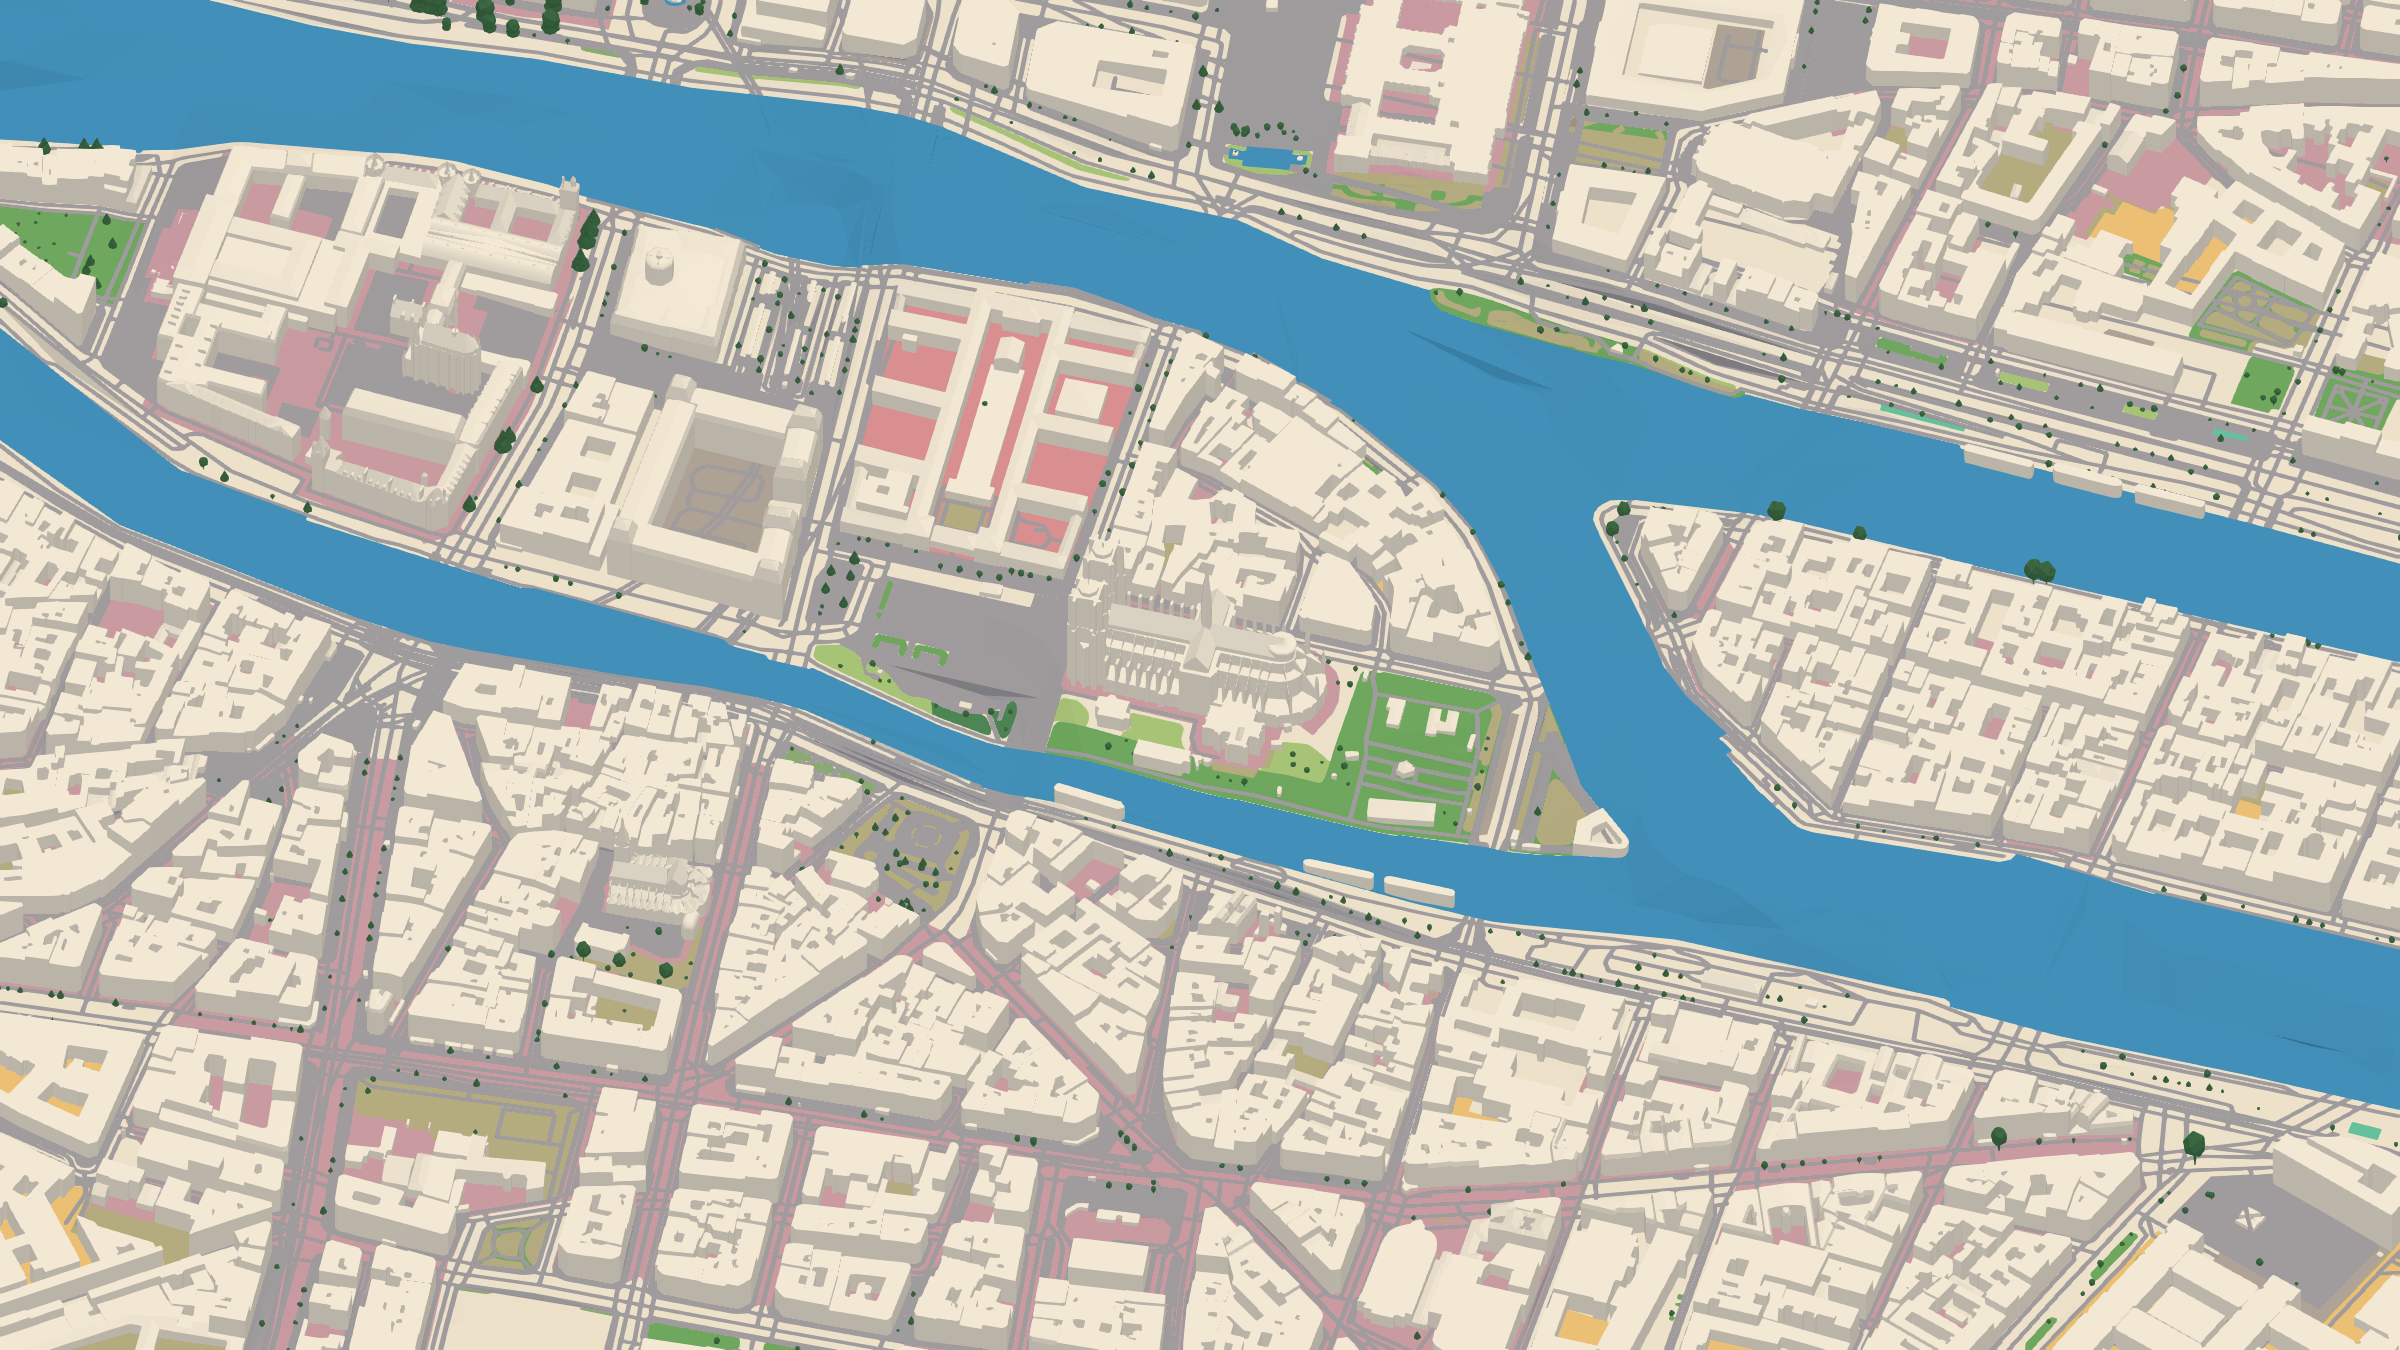
\includegraphics[width=\linewidth]{graphics/ktirio/paris-notre-dame.png}
    \caption{The mesh around Notre-Dame and the Seine.}
  \end{subfigure}
  \caption{Paris geometry for the Discoverer campaign. The mesh distinguishes
  buildings, water, vegetation and other land surfaces. The
  \href{https://exa-ma.numpex.fr/highlights/ktirio-paris-8km.html}{Exa-MA highlight}
  provides a flyover and a solar-mask animation.}
  \label{fig:ktirio-paris-mesh}
\end{figure}

\paragraph{Strasbourg.}
The ensemble varied five envelope parameters and ranked buildings
by indoor degree-hours above 28\,\textdegree C over one week.
Across three independent 128-sample replications, 412 of the 417
buildings in the highest-exposure decile were common to all three.
Independent reconstruction reproduced the streamed statistics and
heat-exposure indicators to numerical precision.
Each production task allocated 97 CPU cores, with 32 simulation ranks
for each of three concurrent samples and one statistical rank.
Up to five tasks ran concurrently, using 485 cores. The full campaign
used 21,813.6 allocated core-hours including the build and qualification
runs (HiDALGO2 D4.10).

The paper accepted for the PPAM 2026 proceedings compares overheating
under paired night-ventilation scenarios with the same weather and
sampled building properties.
In the reported cases, computing degree-hours from the ensemble-mean
temperature underestimated mean exposure. Computing them for each
realisation first preserves the effect of crossing the temperature
threshold \cite{antonczak_ktirio_2026}.

\subsection{Use and next steps}

The heat-exposure ranking shows how the simulations can inform a
shortlist for follow-up under specified conditions. Extending the use
to renovation decisions requires checking the building models against
local observations. The urban microclimate work will assess how
two-way feedback changes the thermal boundary conditions. The next
performance studies will quantify the output cost with field export
enabled and the trade-off between storage and accuracy for ensemble
statistics. Within HiDALGO2, the renewable-energy pilot already
uses Ktirio's panel-level shading in its photovoltaic workflow.
Within NumPEx, Exa-AToW supported deployment on Jean Zay.

\clearpage
\section{FUnTiDES -- Wave Propagation}
\label{sec:pc5:funtides}

\begin{FicheMetadataTable}[FUnTiDES demonstrator profile.]
Domain & Computational geophysics and seismic wave propagation. \\
Application team & Inria Makutu and an industrial partner in the energy sector. \\
Co-design & Exa-DI's working group on efficient PDE discretisation (WG1)
and the CDT. \\
Exa-MA contributions & WP1 high-order wave discretisation and matrix-free
operators. WP7 benchmarking and co-design coordination. \\
Software and data &
\ExaDIRef{sec:FUnTiDES:software}{FUnTiDES}{https://github.com/FUnTiDES-sim/FUnTiDES}
with a Kokkos C++ backend. Proxy-Fun and Proxy-Kernels for spectral-element operators. \\
Reference cases & Acoustic and elastic operator tests, and a coupled
DG--SEM example in a layered acoustic medium. \\
\end{FicheMetadataTable}

\subsection{Context and objectives}

FUnTiDES models how acoustic and elastic waves propagate through the
subsurface. Resolving those waves in large three-dimensional models
requires repeated application of the discrete operator over many time
steps. The co-design question is how to maintain high-order accuracy
while controlling that cost on GPU-based systems. The
\href{https://numpex.org/wp-content/uploads/sites/6/2026/03/High-Performance-Spectral-Element-Operators-on-GPUs-.pdf}{February 2026 Exa-DI WG1 presentation}
places FUnTiDES among the teams working on this problem. The
\href{https://radar.inria.fr/report/2025/makutu/index.html}{Makutu activity report}
describes earlier acoustic proxy cases and the industrial collaboration.

\subsection{Methods and HPC implementation}

The
\ExaDIRef{sec:FUnTiDES:software}{FUnTiDES software fiche}{https://github.com/FUnTiDES-sim/FUnTiDES}
describes the second-order wave equation and its spectral-element (SEM),
discontinuous Galerkin and coupled DG--SEM discretisations.
\href{https://github.com/FUnTiDES-sim/FUnTiDES/releases/tag/0.2.0}{FUnTiDES 0.2.0}
provides a Kokkos C++ backend for CPUs and GPUs. The
\ExaDIRef{sec:wp1:t1.4}{WP1/T1.4 wave-proxy work}{https://exa-ma.numpex.fr/deliverables.html}
examines matrix-free high-order operators. The CDT in Exa-DI WG1 is
consolidating Proxy-Fun, which covers acoustic and elastic SEM operators,
and Proxy-Kernels, which isolates the operator application. The latter
compares classical quadrature with tensor contractions expressed as
batched dense matrix multiplications (GEMM).

In the layered acoustic example in \cref{fig:exadi-funtides-dgsem},
SEM subdomains use polynomial orders 2, 4 and 6. Thin DG layers
couple subdomains of different orders. The wavefield snapshots show
propagation through the layered medium.

\begin{figure}[H]
  \centering
  \begin{subfigure}[t]{0.485\linewidth}
    \centering
    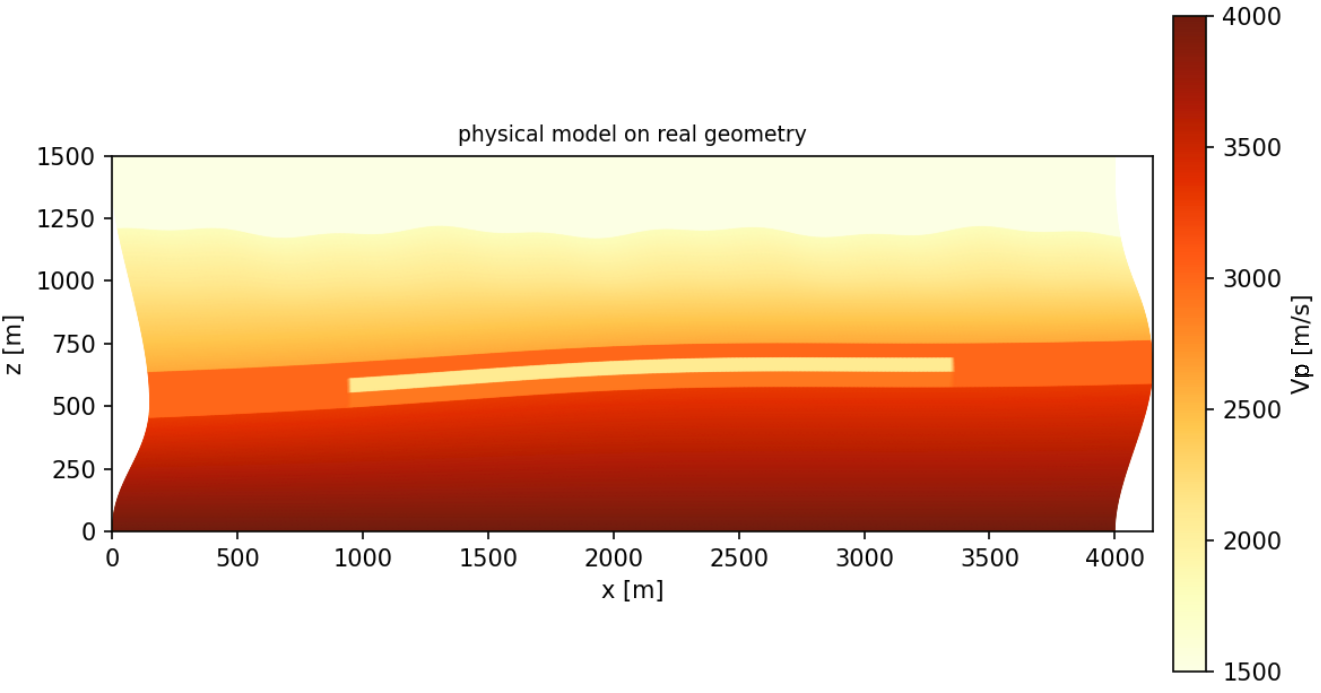
\includegraphics[width=\linewidth]{graphics/funtides/acoustic-model.png}
    \caption{Acoustic wave speed (m/s).}
  \end{subfigure}\hfill
  \begin{subfigure}[t]{0.485\linewidth}
    \centering
    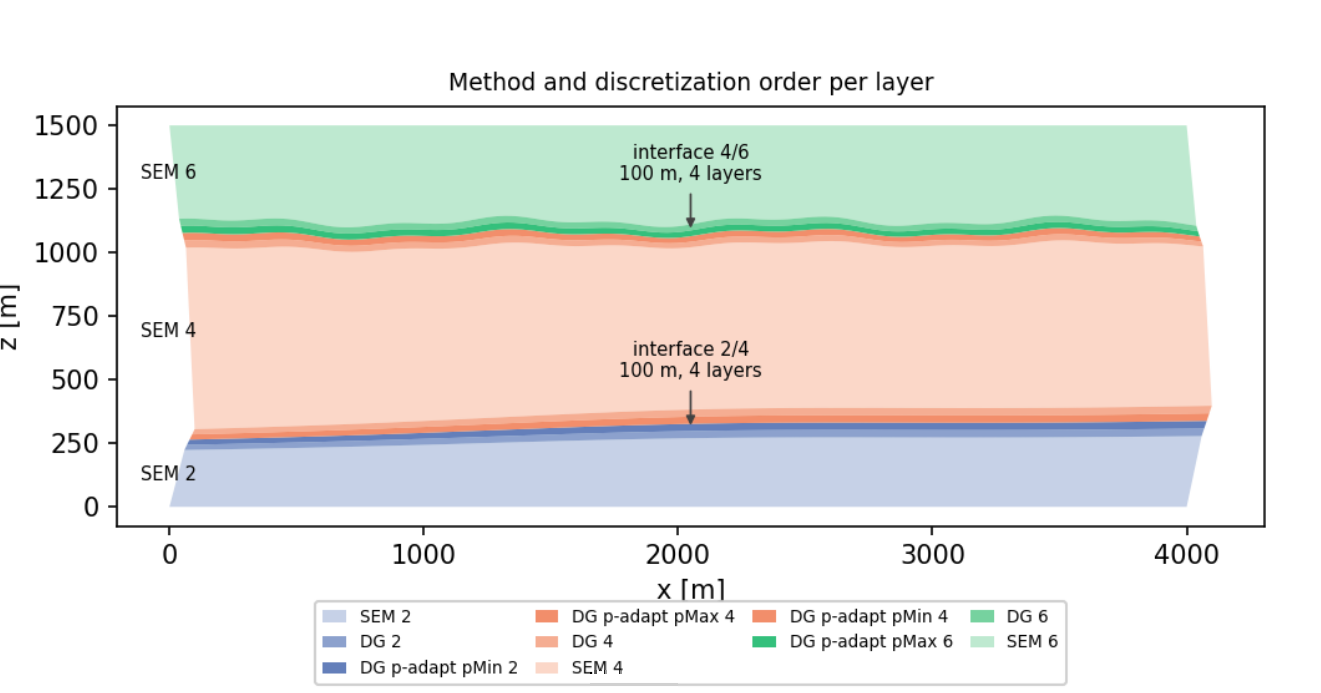
\includegraphics[width=\linewidth]{graphics/funtides/dg-sem-orders.png}
    \caption{SEM orders and DG interfaces.}
  \end{subfigure}
  \par\medskip
  \begin{subfigure}[t]{0.485\linewidth}
    \centering
    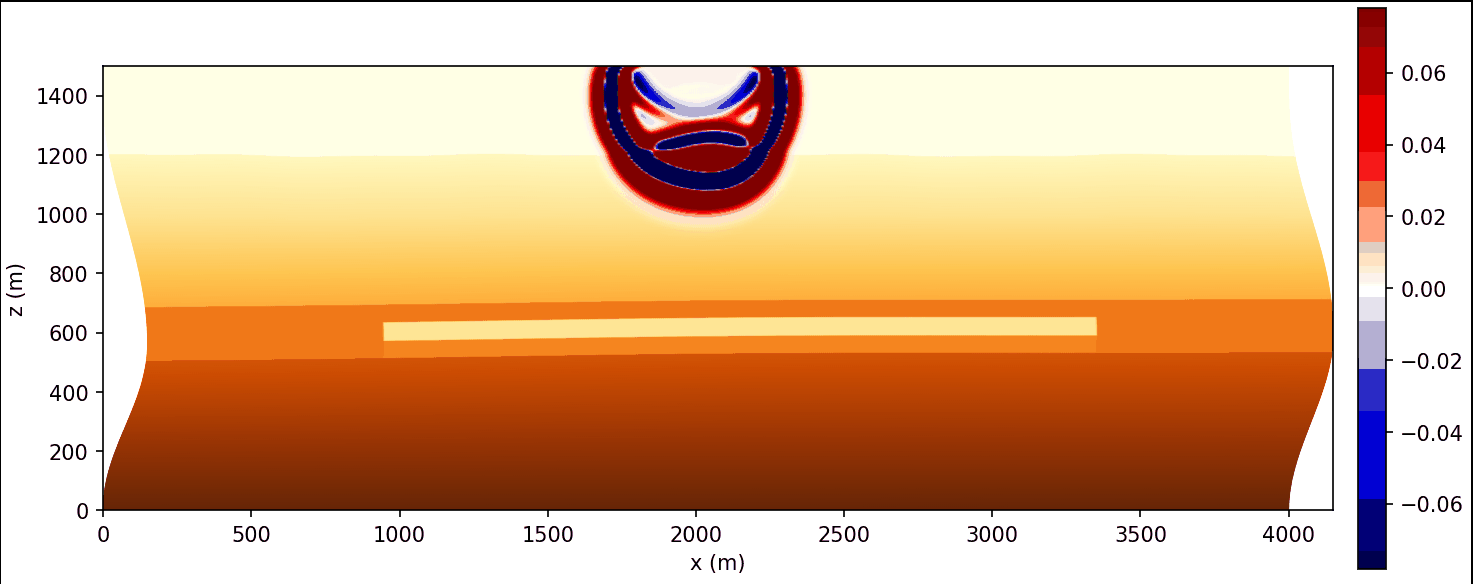
\includegraphics[width=\linewidth]{graphics/funtides/wavefield-early.png}
    \caption{Earlier wavefield snapshot.}
  \end{subfigure}\hfill
  \begin{subfigure}[t]{0.485\linewidth}
    \centering
    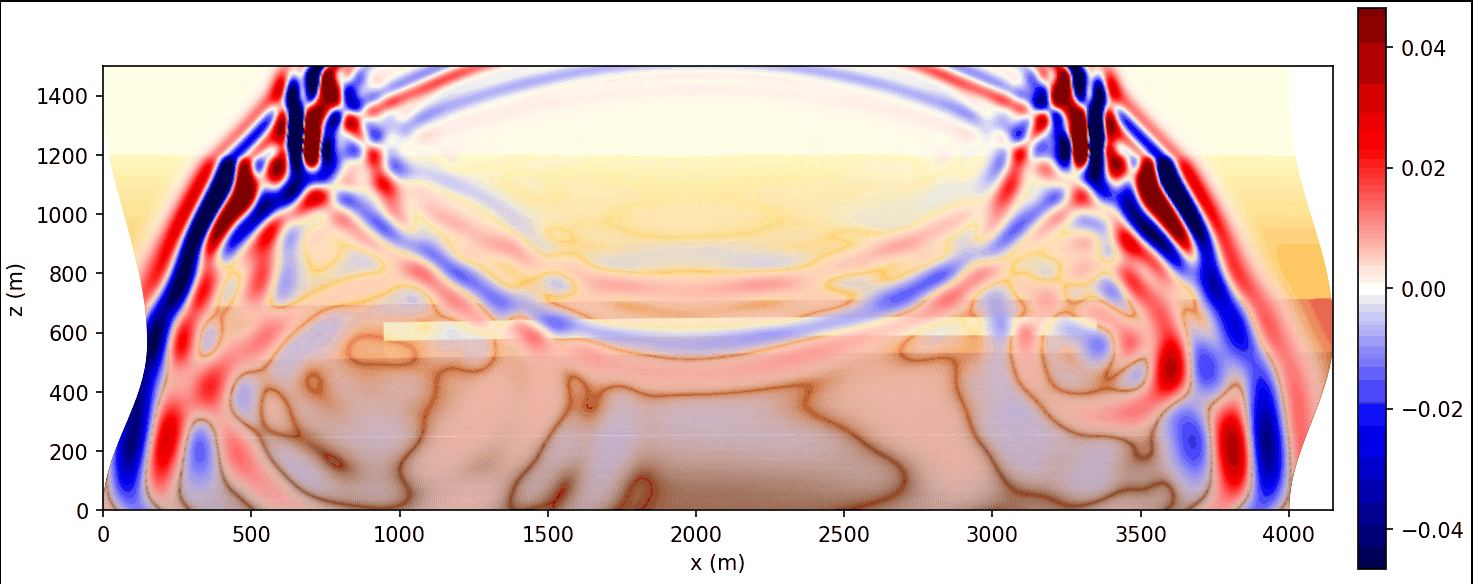
\includegraphics[width=\linewidth]{graphics/funtides/wavefield-late.png}
    \caption{Later wavefield snapshot.}
  \end{subfigure}
  \caption{Coupled DG--SEM simulation in a layered acoustic medium.
  Figures courtesy of Aurélien Citrain (Inria Makutu).}
  \label{fig:exadi-funtides-dgsem}
\end{figure}

\subsection{Results and benchmarks}

% Campaign plans and adoption of the GEMM operator: Aurélien Citrain, Inria, November 2026.
\begin{table}[H]
\centering\small
\caption{Reported and planned wave-propagation benchmarks.}
\label{tab:exadi-funtides-results}
\begin{tabularx}{\linewidth}{@{}>{\raggedright\arraybackslash}p{0.22\linewidth}
  >{\raggedright\arraybackslash}p{0.18\linewidth}
  >{\raggedright\arraybackslash}X@{}}
\toprule
\textbf{Case} & \textbf{Status} & \textbf{Scope and result}\\
\midrule
Proxy-Kernels spectral-element comparison &
Measured on GPU &
The CDT reported shorter runtimes for the tensor/GEMM implementations
at polynomial orders four and five, relative to classical quadrature
in the tested configurations. FUnTiDES has adopted the GEMM operator.\\
\addlinespace
FUnTiDES seismic simulations on Alice Recoque &
Planned &
Two synthetic seismic cases are being prepared for multi-GPU and
multi-node runs targeting more than one billion degrees of freedom.
Higher polynomial orders will also be considered.\\
\bottomrule
\end{tabularx}
\end{table}

\subsection{Use and next steps}

The planned seismic cases extend the operator measurements to the
distributed application, where communication and the complete
time-stepping loop also contribute to runtime. They will test
whether the kernel gains carry through to the simulation workload.
Local time stepping is planned for cases where the stability
constraint varies across the mesh.

\clearpage
\section{Samurai -- Adaptive Cartesian Meshes}
\label{sec:pc5:samurai}

% Team input requested: target application and output quantity, full
% adaptive workflow and I/O, measured accuracy-cost trade-off and
% cross-project contributions, scaling results and platform.
\begin{FicheMetadataTable}[Samurai demonstrator profile.]
Domain & Adaptive finite-volume simulation on Cartesian meshes. \\
Application team & HPC@Maths, CMAP, École polytechnique. \\
Co-design & Exa-DI's working group on block-structured adaptive mesh
refinement (WG3), with Dyablo (CEA) and the CDT. \\
Exa-MA contributions & WP1 adaptive discretisation and high-order
coupling verification. WP7 benchmarking coordination. \\
Software and data &
\ExaDIRef{sec:Samurai:software}{Samurai}{https://hpc-math-samurai.readthedocs.io/en/latest/}
and Cwipi for coupling. Adaptive-mesh data and I/O work with
Exa-DoST, and task execution work with Exa-SoFT. \\
Reference cases & Adaptive Burgers, Euler shocks and solid--fluid heat transfer. \\
\end{FicheMetadataTable}

\subsection{Context and objectives}

Shock fronts and other localised structures can require much finer
resolution than the rest of a computational domain. Samurai studies
how to concentrate cells where the solution needs them, and whether the
cost of adapting and redistributing the mesh is offset by the smaller
problem. The
\href{https://numpex.org/wp-content/uploads/sites/6/2026/03/RoadmapWG3.pdf}{Exa-DI WG3 roadmap of 24 February 2026}
identifies Samurai and Dyablo as the working group's two application
teams. Its common reference set includes a non-axis-aligned Sod shock
tube, a Sedov blast and Double Mach Reflection.

\subsection{Methods and HPC implementation}

Samurai represents adaptive Cartesian meshes as intervals of cells and
uses set operations to manipulate them. The
\ExaDIRef{sec:Samurai:software}{software fiche}{https://hpc-math-samurai.readthedocs.io/en/latest/}
describes its multiresolution methods, also applied to adaptive lattice
Boltzmann simulations \cite{bellotti_multiresolution-based_2022}.
The WP1 coupling case uses Cwipi for exchange across a solid--fluid
interface. The
\href{https://exa-ma.numpex.fr/news/2026/20260626-samurai-framework-webinar.html}{June Exa-MA webinar}
describes complementary work with Exa-DoST on adaptive-mesh data and
I/O, and with Exa-SoFT on expressing adaptive computations as StarPU tasks.

\subsection{Results and benchmarks}

\begin{table}[H]
\centering\small
\caption{Samurai cases and their benchmark status in the Exa-MA collection.}
\label{tab:exadi-samurai-results}
\begin{tabularx}{\linewidth}{@{}>{\raggedright\arraybackslash}p{0.23\linewidth}
  >{\raggedright\arraybackslash}p{0.20\linewidth}
  >{\raggedright\arraybackslash}X@{}}
\toprule
\textbf{Case} & \textbf{Status} & \textbf{Scope and result}\\
\midrule
\ExaDIRef{sec:app:specs:app-samurai-burgers-2d}{Adaptive 2D Burgers}{https://github.com/hpc-maths/samurai} &
Executable &
MPI case tested in CI on two to nine processes.
Weak-scaling measurements pending
(\nolinkurl{BM-SAMURAI-BURGERS-01}).\\
\addlinespace
\ExaDIRef{sec:app:specs:app-samurai-euler-dmr}{Double Mach Reflection}{https://github.com/hpc-maths/samurai-euler} &
Executable &
Euler case records timings for strong-scaling and scaled-resolution
series. Scaling measurements pending
(\nolinkurl{BM-SAMURAI-DMR-01}).\\
\addlinespace
\ExaDIRef{sec:app:specs:app-samurai-cwipi}{Samurai--Cwipi heat transfer}{https://exa-ma.numpex.fr/deliverables.html} &
Convergence measured &
The multistep coupling scheme achieved the predicted temporal
convergence through order four on the solid--fluid reference case.\\
\bottomrule
\end{tabularx}
\end{table}

\subsection{Use and next steps}

The common Euler cases will compare solution error and total runtime
as resolution and process count increase. The coupling study provides
a reference for checking accuracy when adaptive discretisations are
used in multiphysics workflows.
